\nonstopmode

%\documentclass[twoside]{pwrthesis}
\documentclass[oneside]{iisthesis}
% ---
%\usepackage[MeX]{polski}
%\usepackage[polish]{babel}
%\usepackage[cp1250]{inputenc}

\usepackage{polski}
\usepackage[polish]{babel}
\usepackage[utf8]{inputenc}
\usepackage{graphicx}

% Dodane przeze mnie d
\usepackage{fancyvrb} % dla srodowiska Verbatim
\usepackage{color}
\usepackage{lscape}
\usepackage{amssymb}

\usepackage{icomma}
\usepackage{placeins}

% definicje kolorow
\definecolor{ciemnoSzary}{rgb}{0.15,0.15,0.15}
\definecolor{szary}{rgb}{0.5,0.5,0.5}
\definecolor{jasnoSzary}{rgb}{0.2,0.2,0.2}

% Konfiguracja verbatima
\fvset{
	frame=single,
	numbers=left,
	fontsize=\footnotesize,
	numbersep=12pt,
%	framerule=.5mm,
	rulecolor=\color{ciemnoSzary},
%	fillcolor=\color{jasnoSzary},
	framesep=4pt,
	stepnumber=1,
	numberblanklines=false,
	tabsize=2,
%	formatcom=\color{szary}
}

\begin{document}

\title{Opracowanie inteligentnego systemu sterowania ruchem drogowym.}
\author{inż. Przemysław Rokosz}
\advisor{dr inż. Grzegorz Filcek}
\instituteLogo{logos/pwr}
\slowaKluczowe{pierwsze\\drugie\\trzecie}

\date{\number\the\year}

% Wstawienie abstractu pracy
	%\input {abstract}
	
\abstractSH{
Bardzo krótkie streszczenie w którym powinno się znaleźć omówienie tematu pracy i poruszanych terminów. Tekst ten nie może być zbyt długi. }

\abstractPL{
	AbstraktPL
}
\abstractEN{
	AbstraktEN
}

\maketitle
\textpages

%\chapter*{Wprowadzenie}

%chapter -> section -> subsection

\chapter{Wstęp}
\section{Wprowadzenie}
Inteligentne systemy sterowania ruchem drogowym są aktualnym trendem rozwoju miejskiej infrstruktury drogowej w Polsce i stale zyskują na popularności.
Systemy takie tworzone są częściowo w opraciu o istniejącą infrastrukturę i pozwalają na optymalizację przepływu pojazdów w sterowanym obszarze.
Celami stawianymi systemom kontroli ruchu drogowego są: skrócenie czasu podróży, zwiększenie bezpieczeństwa czy poprawa komfortu podróży.

Kontrola ruchu drogowego może być oparta, w zależności od celów stawianych systemowi, o maksymalizację wykorzystania sieci drogowej jak i minimalizację czasu przejazdów. Częstym celem, zastosowania inteligentnych systemów sterowania, jest poprawa warunków ruchu pojazdów komunikacji zbiorowej, nawet jeśli prowadzi to do zmniejszenia priorytetu ruchu pojazdów indywidualnych.

Rozwiązanie problemu sterowania ruchem może opierać się o systemy uczące się czy systemy wykorzystujące metody optymalizacyjne. W poniższej pracy przedstawiona została próba stworzenia systemu sterowania ruchem drogowym w oparciu o algorytm sterowania wykorzystujący matematyczny model ruchu drogowego.

\section{Cel pracy}
Celem niniejszej pracy jest próba opracowania systemu sterowania ruchem drogowym na obszarze wzorowanym na okolicach placu Grunwaldzkiego we Wrocławiu. Przygotowany algorytm sterowania zostanie porównany z zachowaniem ruchu drogowego w przypadku braku sterowania jak i przy zastosowaniu stałego, niezsynchronizowanego, programu, stałoczasowej sygnalizacji świetlnej.

Motywacją w powstaniu tej pracy jest próba stworzenia systemu który będzie dynamicznie reagował na zmienną charakterystykę ruchu drogowego oraz będzie stosował się do, wymaganych przez prawo, ograniczeń.

\chapter{Przegląd literatury}
\section{Wymagania prawne dotyczące sygnalizacji świetlnej}
Podstawowe zasady projektowania sygnalizacji świetlnej oraz jej programów opisuje Rozporządzenie Ministra Infrastruktury z dnia 3 lipca 2003 roku \cite{rozporzadzenie}.
Ze względu na tematykę pracy, najważniejszy jest załącznik nr 3 rozporządzenia opisujący szczegółowe warunki techniczne dla sygnałów drogowych w tym wymagania dotyczące programu sygnalizacji świetlnej w punkcie ósmym.
Wymagania programu sygnalizacji zaczynają się od zasad ogólnych, opisujących między innymi programy przejściowe z i do sygnału ostrzegawczego (oznaczającego wyłączenie sygnalizacji). Następnie opisane są wymagania formalne w tym wymagania czasowe dotyczące sygnałów, opisane dokładniej w rozdziale \ref{sec:model_ograniczenia}. na stronie \pageref{sec:model_ograniczenia}.
W dalszej części opisane są wymagania bezpieczeństwa ruchu w tym metoda wyliczenia długości czasów międzyzielonych, czyli odstęp czasu służący zabezpieczeniu aby pojazdy poruszające się w kolizyjnych strumieniach ruchu nie znalazły się w tym samym miejscu i czasie. Metoda wyliczania czasów międzyzielonych również opisana jest w rozdziale \ref{sec:model_ograniczenia}.

\section{Metody stosowane w sterowaniu ruchem drogowym}
Usystematyzowany przegląd metod i algorytmów sterowania ruchem drogowym przedstawiają w swojej pracy Piotr Kawalec z Politechniki Warszawskiej oraz Sylwia Sobieszuk\-Durka z Urzędu m. st. Warszawy \cite{kawalec+sobieszuk-durka}. Dzielą oni metody sterowania ruchem drogowym na optymalizujące i nieoptymalizujące funkcji celu.
Przedstawione wartości optymalizowane mogą być wprost zastosowane do oceny opracowywanego systemu sterowania ruchem drogowym.

Autorzy zauważają, że nawet najlepszy algorytm sterowania ruchem nie da dobrych efektów jeśli zostanie zastosowany dla pojedynczego skrzyżowania. Stąd konieczne jest opracowanie systemów sterowania z myślą o większych zespołach w których sygnał sterujący wpływa na wiele miejsc w zakresie rozpatrywanego obszaru.

We wspomnianej pracy przedstawione zostały przykładowe struktury systemów adaptacyjnego sterowania ruchem drogowym co jest dobrym punktem wyjścia do projektowania inteligentnego systemu sterowania ruchem. Opracowana w ramach tej pracy struktura sterowania opisana została w rozdziale \ref{sec:model_opis} na stronie \pageref{sec:model_opis}.

W swojej rozprawie doktorskiej \cite{ruchaj} Marcin Ruchaj przytacza algorytmy sterowania ruchem drogowym z podziałem na sterowanie stałoczasowe - ze stałym programem sygnalizacji, zmiennoczasowe - adaptujące się do warunków ruchu, oraz sterowanie wykorzystujące logikę rozmytą czy metody sztucznej inteligencji, przedstawione również w pracy Tahere Royani Javad Haddadni i Mohammada Alipoora \cite{royani+haddadnia+alipoor}. W swoim referacie proponują oni zastosowanie rozmytych sieci neuronowych do sterowania ruchem i algorytmu genetycznego w celu regulacji parametrów pracy sieci neuronowej.

\section{Rozwiązania w symulacji ruchu drogowego}
Dla celów symulacji ruchu drogowego często wykorzystywane są automaty komórkowe. Zaletą zastosowania automatów komórkowych jest ich oparcie o proste zasady i wysoka wydajność obliczeniowa. Popularny model symulacji ruchu pojazdów opracowali Kai Nagel i Michael Schreckenberg w roku 1992 \cite{nasch}. We wspomnianej pracy opisują oni automat komórkowy którego działanie opiera się na 4 etapach: przyśpieszeniu, hamowaniu, losowości i przesunięciu. Zastosowanie automatów komórkowych w symulacji różnych sytuacji ruchu drogowego opisuje w swojej pracy dyplomowej Maciej Bartodziej \cite{bartodziej}.

Ze względu na swoją prostotę automaty komórkowe można również prosto modyfikować. Przykład symulacji ruchu drogowego w zmiennych warunkach pogodowych przedstawiają w swoim artykule Marcin Bernaś i Bartłomiej Płaczek \cite{bernas+placzek}. Dla celu niniejszej pracy opracowany został symulator stosujący automat komórkowy zmodyfikowany w celu umożliwienia symulacji zespołów skrzyżowań, dokładny opis automatu i jego modyfikacji znajduje się w rozdziale \ref{chap:symulacja} na stronie \pageref{chap:symulacja}.

\section{Istniejące systemy sterowania ruchem}
Inteligentne systemy transportu (ITS\footnote{intelligent transportation systems}) zyskują coraz większą popularność w zarządzaniu ruchem drogowym.
Mają one na celu skrócenie czasu podróży, poprawę bezpieczeństwa czy zwiększenie komfortu podróży co w swojej prezentacji, przedstawiające innowacje w zarządzaniu transportem miejeskim zauważają Aneta Pluta-Zarembska, Marzenna Cichosz i Katarzyna Nowicka ze Szkoły Głównej Handlowej w Warszawie \cite{pluta-zaremba+cichosz+nowicka}. Jako przykład wdrożenia ITS przedstawiony został inteligentny system zarządzania transportem we Wrocławiu. Cel Wrocławskiego systemu, przyspieszenie ruchu o 20\%,  ma zostać osiągnięty, do III kwartału 2014 roku, dzięki zastosowaniu sterowania ruchem na 153 skrzyżowaniach, usprawnieniu komunikacji miejskiej czy dynamicznych informacjach dla kierowców.

Podobny system, zastosowany w trójmieście, prezentują, w artykule na temat systemu TRISTAR, Kazimierz Jamroz i Jacek Oskarbski \cite{jamroz+oskarbski}. Jak zauważają, motywacją wprowadzenia systemu jest między innymi: zatłoczenie infrastruktury drogowej, ryzyko zdarzeń drogowych czy brak informacji o warunkach ruchu. System TRISTAR składa się z połączonych komponentów, takich jak:
\begin{itemize}
	\item zarządzanie ruchem drogowym
	\item zarządzanie transportem zbiorowym
	\item zarządzanie służbami ratowniczymi
	\item zintegrowany system informacji
	\item zarządzanie transportem towarowym
\end{itemize}
Zarządzenie ruchem drogowym obejmuje zarządzanie ruchem miejskim jak i ruchem na okolicznych drogach krajowych i szybkiego ruchu (w postaci trójmiejskiej obwodnicy).

Kolejnym przykładem systemu wdrażanego w Polsce jest podhalański system sterowania ruchem, przedstawiony w artykule Patryka Zakrzewskiego dla magazynu \textit{Drogi Budownictwo Infrastrukturalne} \cite{zakrzewski}. Podobnie jak w przypadku poprzednich dwóch systemów, celami systemu jest zwiększenie bezpieczeństwa i zmniejszenie zatłoczenia na drogach. Jednakże, w przeciwieństwie do nich, podhalański system projektowany był z myślą o zastosowaniu poza warunkami miejskimi. Jego głównym elementem jest monitoring dróg regionu oraz przedstawienie kierowcom informacji o czasie przejazdu do miejscowości orientacyjnych. Jest to więc typowy system proaktywny, działający przed powstaniem zatorów drogowych, w przeciwieństwie do systemów reaktywnych, reagujących na aktualną systuację na drodze. Przykładami systemów reaktywnych są elementy zaprezentowanych wcześniej systemów Wrocławskiego i Trójmiejskiego. Opracowywany w ramach tej pracy system również jest przykładem systemu reaktywnego.

\chapter{Model sterowania ruchem drogowym}
\label{chap:model}
Przyjęty model sterowania zakłada, że system sterowania ruchem drogowym jest systemem dyskretnym. Podobnie, przyjęty model symulatora w postaci automatu komórkowego zakłada symulację ruchu w postaci dyskretnych stanów. Długość każdego stanu to jedna sekunda co daje jedną sekundę na wyznaczneie nowego stanu sygnalizatorów na podstawie akutalnego stanu czujników.

Obszar, obiekt, sterowania udostępnia dane kontrolerom w postaci wartości dwóch typów czujników. Czujnika przepływu pojazdów na dojeździe do sygnalizatora, w którym przepływ wyznaczany jest na podstawie liczby pojazdów mijających czujnik w zadanym czasie, oraz czujnika kolejki. Długość kolejki wyznaczana jest jako liczba pojazdów znajdujących się na wybranym odcinku drogi w danej chwili czasu.

Kontroler wpływa na sterowany obszar przez zmianę stanu sygnalizatorów. Pojazdy reagują na stan sygnalizatora mijając go jedynie jeśli zezwala on na przejazd.

\section{Model sterowania}
\label{sec:model_opis}

Na rysunku \ref{fig:model} zaprezentowany został ogólny model sterowania ruchem drogowym.
Zespół skrzyżowań objęty sterowaniem podzielony jest na obszary.
Każdy obszar obejmuje pojedyncze skrzyżowanie lub jego autonomiczną część, czyli taką w której dojazd strumieni ruchu do miejsca przecięcia jest kontrolowany bezpośrednio jedynie przez sygnalizatory znajdujące się w danej części skrzyżowania.

Każdy obszar sterowany jest przez pojedynczy kontroler.
Kontroler jako dane wejściowe przyjmuje stan systemu w poprzedniej chwili czasu,
zawierający wielkości mierzone przez czujniki jak i sterowania wszystkich kontrolerów. Zapewnia to możliwość współpracy sąsiadujących kontrolerów.

Powyższy, uproszczony, model ograniczony jest do sterowania jednym typem pojzadów. Nie uwzględnia on również sterowania ruchem pieszych i rowerzystów na przjściach dla pieszych oraz przejazdach dla rowerów. W tak zdefiniowanym modelu można przyjąć, że sygnalizatory dla pieszych i rowerzystów, nadają sygnał zezwalający (zielony) w czasie gdy przecinające potoki ruchu otrzymują sygnał czerwony.
Aby zapewnić że sytuacja tego typu jest możliwa należy wymusić przynajmniej jednorazowe, dla każdego sygnalizatora, użycie sygnału czerwonego, zgodnie z ograniczeniami opisanymi w sekcji \ref{sec:model_ograniczenia}.

\begin{figure}[h]
    \centering
    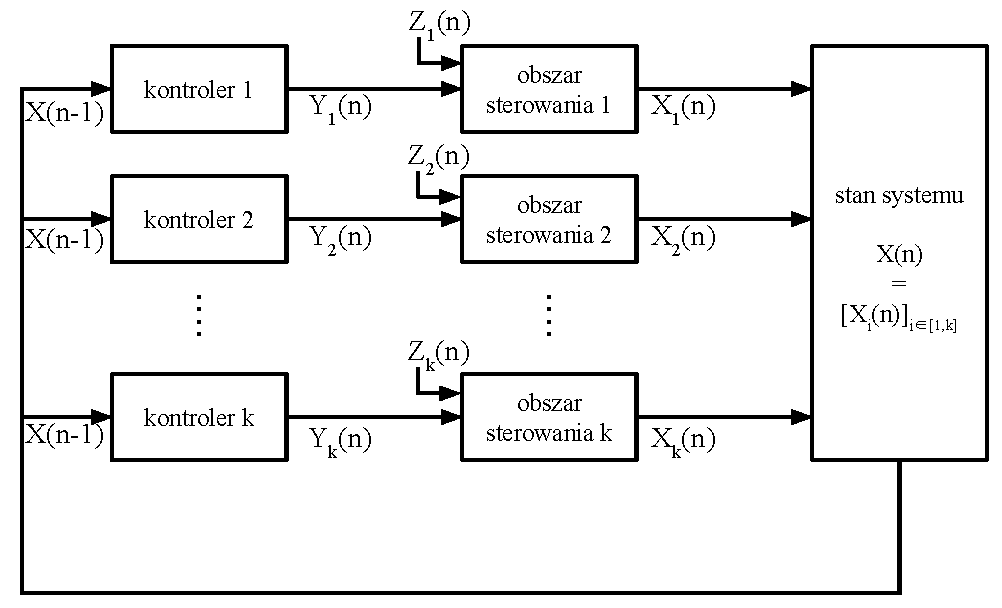
\includegraphics[width=0.8\textwidth]{images/model.pdf}
    \caption{Model systemu sterowania}
    \label{fig:model}
\end{figure}

\begin{equation}
	\begin{array}{c}
		U_i (n) = \left[ u_{i, j} (n) \right]_{j \in <1,s>}\\
		i \in <1,o>\\
		u_{i, j} (n) \in \left\{ \textrm{CZERWONY, CZERWONO-ZOLTY, ZIELONY, ZOLTY} \right\}\\
		o \in \mathbb{N}\\
		s \in \mathbb{N}
	\end{array}
\end{equation}

u_{i,j} (n) \textrm{ -- stan j-tego sygnalizatora w i-tym obszarze w chwili n}

o -- liczba obszarów sterowania

s -- liczba sygnalizatorów w obszarze

\begin{equation}
	\begin{array}{c}
		Z_i (n) = \left[ z_{i, j} (n) \right]_{j \in <1,r>}\\
		i \in <1,o>\\
		z_{i, j} (n) \in \mathbb{N}\\
		r \in \mathbb{N}
	\end{array}
\end{equation}

z_{i,j} (n) \textrm{ -- przepływ pojazdów z kierunku j w i-tym obszarze w chwili n}

r -- liczba wlotów do danego obszaru sterowania

\begin{equation}
	\begin{array}{c}
		X_i (n) = \left[
			\begin{array}{c}
				x_{i, j, 1} (n) \\ x_{i, j, 2} (n) \\ x_{i, j, 3} (n)
			\end{array}
		\right]_{j \in <1,s>}\\
		i \in <1,o>\\
		x_{i, j, 1} (n) \in \mathbb{N}\\
		x_{i, j, 2} (n) \in \mathbb{N}\\
		x_{i, j, 3} (n) \in \left\{ \textrm{CZERWONY, CZERWONO-ZOLTY, ZIELONY, ZOLTY} \right\}
	\end{array}
\end{equation}

x_{i, j, 1} (n) \textrm{ -- przepływ na dojeździe do j-tego sygnalizatora w i-tym obszarze}

x_{i, j, 2} (n) \textrm{ -- kolejka przed j-tym sygnalizatorem w i-tym obszarze}

x_{i, j, 3} (n) \textrm{ -- stan j-tego sygnalizatora w i-tym obszarze}

\vspace{0.5cm}
Przepływy pojazdów mierzone są w pojazdach na godzinę, stany kolejek mierzone są w postaci liczby pojazdów.

\section{Wymagania sterowania ruchem drogowym}
\label{sec:model_ograniczenia}
Ograniczenia dotyczące sterowania ruchem drogowym zostały ustalone w rozporządzeniu ministra infrastruktury \cite{rozporzadzenie}. Wymagania te można sprowadzić do zestawu wymagań formalnych i wymagań bezpieczeństwa:
\subsection{Wymagania formalne}
\begin{itemize}
	\item Sekwencja sygnałów czerwony, czerwono-żółty\footnote{sygnał czerwony z żółtym, przygotowanie do jazdy}, zielony, żółty, czerwony
	\item Długość sygnału żółtego powinna wynosić 3 sekundy
	\item Długość sygnału czerwono-żółtego powinna wynosić 1 sekundę
	\item Dla sygnalizacji akomodacyjnej/acyklicznej minimalna długość sygnału zielonego to 5 sekund
\end{itemize}

\subsection{Wymagania bezpieczeństwa}
Rozporządzenie definiuje podział par strumieni ruchu na strumienie niekolizyjne, strumienie kolizyjne o dopuszczalnym jednoczesnym zezwoleniu na ruch oraz strumienie kolizyjne o niedopuszczalnym jednoczesnym zezwoleniu na ruch. Ze względów bezpieczeństwa, na potrzeby opracowywanego systemu przyjęto, że strumienie kolizyjne nigdy nie mogą otrzymać jednoczesnego zezwolenia na ruch.

Zdefiniowano metodę obliczania czasów międzyzielonych dla kolizyjnych par strumieni. Zapewniają one minimalny czas w którym strumień ewakuujący się zdąży minąć punkt kolizji zanim osiągnie go strumień dojeżdżający. Minimalny czas międzyzielony wyznacza się na podstawie czasu trwania sygnału żółtego dla strumienia ewakuującego się, czasu ewakuacji strumienia ewakuującego się oraz czasu dojazdu strumienia dojeżdżającego.

\begin{equation}
	t^{min}_{m} (i,j) = t_{z} + t_{e} (i,j) - t_{d} (i,j)
\end{equation}

t^{min}_{m} (i,j) \textrm{ -- minimalny czas międzyzielony dla pary strumieni (i,j) [s]}

t_{z} \textrm{ -- długość sygnału żółtego dla strumienia ewakuującego się [s]}

t_{e} (i,j) \textrm{ -- czas ewakuacji strumienia i poza punkt kolizji ze strumieniem j [s]}

t_{d} (i,j) \textrm{ -- czas dojazdu strumienia j do punktu kolizji ze strumieniem i [s]}

t^{min}_{m} (i,j) = 0 \textrm{ jeśli obliczona wartość jest mniejsza od 0}

\begin{equation}
	t_{e} (i,j) = \frac{s_{e} (i,j) + I_p}{v_{e} (i)}
\end{equation}

s_{e} (i,j) \textrm{ -- droga strumienia ewakuującego się od linii zatrzymania do punktu kolizji[m]}

I_p \textrm{ -- wartość wydłużająca drogę ewakuacji, dla strumienia pojazdów 10 metrów}

v_{e} (i) \textrm{ -- prędkość ewakuacji [m/s], prędkość dopuszczalna na wlocie, nie większa niż 14 m/s}

\begin{equation}
	t_{d} (i,j) = \frac{s_{d} (i,j)}{v_{d} (j)} + 1
\end{equation}

s_{d} (i,j) \textrm{ -- droga strumienia dojeżdżającego od linii zatrzymania do punktu kolizji [m]}

v_{d} (i) \textrm{ -- prędkość ewakuacji [m/s], prędkość dopuszczalna na wlocie}

\section{Algorytm sterowania ruchem drogowym}
\begin{figure}[h]
    \centering
    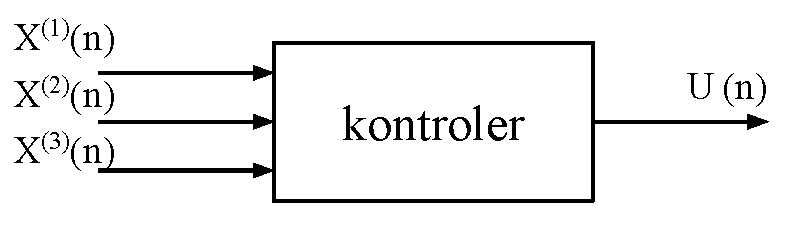
\includegraphics[width=0.5\textwidth]{images/kontroler.pdf}
    \caption{Model sterowania kontrolera}
    \label{fig:kontroler}
\end{figure}

Jak widać na rysunku \ref{fig:model} i \ref{fig:kontroler}, kontroler, do wyznaczenia stanu sygnalizatorów wykorzystuje, stan obiektu sterowanego. Stan obiektu składa się z trzech zmiennych.

\vspace{1.5cm}
\textbf{Parametry algorytmu}

p \in <0.0, 1.0> \textrm{ -- wpływ przewidywanego przepływu pojazdów na sterowanie}

q \in <0.0, 1.0> \textrm{ -- wpływ aktualnego przepływu pojazdów na sterowanie}

r \in <0.0, 1.0> \textrm{ -- wpływ aktualnych wielkości kolejek na sterowanie}

\vspace{1.5cm}
\textbf{Stałe algorytmu}

s \in \mathbb{N} \textrm{ -- liczba sygnalizatorów w kontrolowanym obszarze}

m \in \mathbb{N} \textrm{ -- maksymalny możliwy do zmierzenia przepływ pojazdów}

\begin{equation}
	\begin{array}{c}
		K = \left[ k_{i} \right]_{i \in <0,s>}\\
		k_{i} \in \mathbb{N}
	\end{array}
\end{equation}

k_{i} \textrm{ -- maksymalna możliwa wielkość kolejki przed i-tym sygnalizatorem}

\vspace{1.5cm}
\textbf{Zmienne stanu}

\begin{equation}
	\begin{array}{c}
		X^{(1)} (n) = \left[ x^{(1)}_{i} (n) \right]_{i \in <0,s>}\\
		x^{(1)}_{i} (n) \in \mathbb{N}
	\end{array}
\end{equation}

x^{(1)}_{i} (n) \textrm{ -- przewidywany przyszły przepływ pojazdów w kierunku i-tego sygnalizatora}

Przewidywany przepływ pojazdów jest wyznaczany na podstawie stanu sygnalizatorów sąsiadujacych kontrolerów.

\begin{equation}
	\begin{array}{c}
		X^{(2)} (n) = \left[ x^{(2)}_{i} (n) \right]_{i \in <0,s>}\\
		x^{(2)}_{i} (n) \in \mathbb{N}
	\end{array}
\end{equation}

x^{(2)}_{i} (n) \textrm{ -- przepływ pojazdów w kierunku i-tego sygnalizatora w chwili n}

\begin{equation}
	\begin{array}{c}
		X^{(3)} (n) = \left[ x^{(3)}_{i} (n) \right]_{i \in <0,s>}\\
		x^{(3)}_{i} (n) \in \mathbb{N}
	\end{array}
\end{equation}

x^{(3)}_{i} (n) \textrm{ -- wielkość kolejki przed i-tym sygnalizatorem w chwili n}

\vspace{1.5cm}
\textbf{Algorytm}

Proponowany jest poniższy algorytm wyznaczania nowego stanu sygnalizatorów.
\begin{enumerate}
	\item wyznaczenie wszystkich, zbiorów bezkolizyjnych stanów sygnalizatorów
	\item wyliczenie wag sygnalizatorów
	\item wyliczenie funkcji oceny jako sumy wag sygnalizatorów zezwalających na wjazd dla wyznaczonych wcześniej zbiorów
	\item wyznaczenie optymalnego, o najwyższej wartości funkcji oceny, stanu
\end{enumerate}

\vspace{0.5cm}
W pierwszym kroku algorytmu wyznaczane są wszystkie możliwe zbiory bezkolizyjnych stanów sygnalizatorów.
Spośród tak wyznaczonych zbiorów możliwy jest późniejszy wybór takiego który będzie w danym momencie optymalny.

\vspace{0.5cm}
Kolejny krok pozwala wyznaczyć wagi zezwolnia na ruch przez każdy z sygnalizatorów.

\begin{equation}
	w_{i} (n) = p \cdot \frac{x^{(1)}_{i} (n)}{m} + q \cdot \frac{x^{(2)}_{i} (n)}{m} + r \cdot \frac{x^{(3)}_{i} (n)}{k_{i}}
\end{equation}

w_{i} (n) \textrm{ -- waga i-tego sygnalizatora w chwili n}

\vspace{0.5cm}
W następnym kroku, wyliczone wagi są sumowane aby wyznaczyć wartość funkcji oceny dla każdego, przygotowanego w pierwszym kroku, zbioru.

\begin{equation}
	Q (X(n), S') = \sum\limit_{i \in S'} w_{i}
\end{equation}

S' \textrm{ -- wyznaczony zbiór sygnalizatorów}

\vspace{0.5cm}
Na końcu wybierany jest stan optymalny, o najwyższej funkcji oceny.

\section{Uwzględnienie ograniczeń cyklów świetlnych}
Podstawowym ograniczeniem, spośród wymienionych w rozdziale \label{sec:model_ograniczenia}, jakiego nie uwzględnia tak zdefiniowany algorytm jest ograniczenie faz cyklu świetlnego. Jak już zostało wspomniane  sygnały mogą być nadawane jedynie w zadanej sekwencji. Natomiast powyższy model podejmuje jedynie decyzję o wydaniu zgody na ruch.

Za przestrzeganie tego jak i innych, czasowych, ograniczeń odpowiada dodatkowy komponent który przekazuje do obiektu sterowanego ostateczną decyzję. Zmiana sygnału powoduje utworzenie, przez ten komponent, sekwencji sygnałów które nastąpią w kolejnych chwilach czasu, dodatkowo uruchomienie sygnału zielonego jest odpowiednio opóźnione przez uwzględnienie czasów międzyzielonych. Również ograniczenia długości sygnałów żółtego i czerwono-żółtego są uwzględniane na tym etampie. Wspomniany komponent odpowiada również za wymuszenie uruchomienia sygnału czerwonego przynajmniej raz na cykl świetlny.

\section{Metody oceny skuteczności algorytmu}
Do oceny skuteczności algorytmu wykorzystać można określone na podstawie pracy Piotra Kawalca i Sylwii Sobieszuk-Durki \cite{kawalec+sobieszuk-durka} metody oceny. Są to:
\begin{itemize}
	\item średnie czasy przejazdu pojazdów na wybranych kierunkach
	\item liczba zatrzymań pojazdów
	\item średnia prędkość pojazdów
\end{itemize}

W ten sposób określone metody oceny można wykorzystać do porównania algorytmu z przypadkiem braku sterowania czy sterowaniem przy użyciu prostego, stałoczasowego, niezsynchronizowanego, programu sygnalizacji. Ocena wyników badań znajduje się w rozdziale \ref{chap:ocena}.

\chapter{System sterowania ruchem drogowym}
System, przygotowany do badania algorytmu sterowania, składa się z trzech podstawowych komponentów:
\begin{description}
	\item[symulator] --
		symuluje ruch drogowy, udostępnia dane z czujników i przyjmuje ustawienia sygnalizatorów.
		Jest on również źródłem czasu co pozwala na synchronizację działania całego systemu. Opisany w sekcji \ref{chap:symulacja}.
	\item[kontroler] --
		osobny dla każdego obszaru, otrzymuje dane z symulatora i wyznacza sterowania sygnalizatorów.
		Może komunikować się z innymi kontrolerami w celu wymiany danych o sąsiednich obszarach. Więcej w sekcji \ref{chap:kontroler}.
	\item[serwer] --
		zapewnia abstrakcję komunikacji. Pozwala na wymiane wiadomości w postaci zdarzeń.
		Działanie komunikacji w systemie opisane jest w sekcji \ref{chap:komunikacja}.
\end{description}

\section{Technologia}
System został przygotowany przy użyciu języka C++ w standardzie C++03 z wykorzystaniem biblioteki Boost 1.55.0 \cite{boost}. Do komunikacji sieciowej wykorzystano bibliotekę Google Protocol Buffer \cite{protobuf}. Przygotowane testy jednostkowe wykorzystują bibliotekę Google Test \cite{gtest}.

Obszar symulowany wczytywany jest z plików XML z opisem w postaci grafowej. Pliki z opisem zawierają również obliczone czasy międzyzielone pomiędzy kolizyjnymi strumieniami ruchu.

\section{Obszar badania algorytmu}
Dla celów badania algorytmu przygotowany został opis obszaru okolic placu Grunwaldzkiego we Wrocławiu, przedstawionego na rysunku \ref{fig:mapa_czysta}.

\begin{figure}[h]
    \centering
    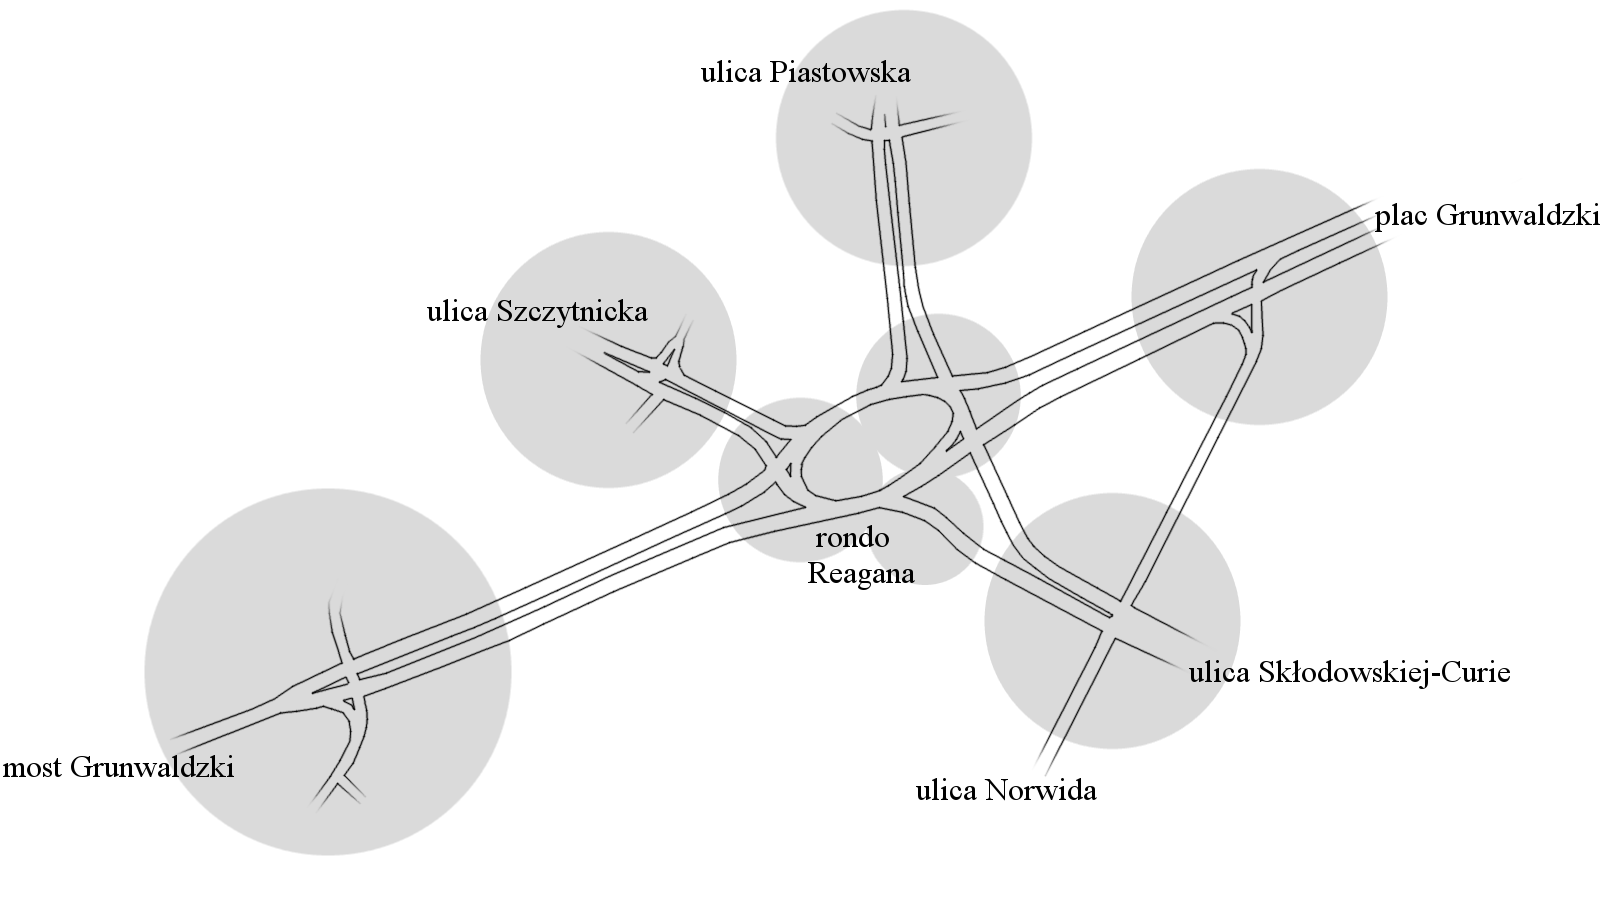
\includegraphics[width=1.0\textwidth]{images/mapa_czysta.png}
    \caption{Mapa obszaru badania algorytmu przedstawiająca okolice placu Grunwaldzkiego we Wrocławiu, przygotowana na podstawie Google Maps \cite{google_maps}}
    \label{fig:mapa_czysta}
\end{figure}

Przygotowany obszar został oparty o rzeczywisty układ drogowy, jednakże został on uproszczony. Uwzględnia on jedynie ruch samochodowy, nie uwzględnia natomiast komunikacji miejskiej czy ruchu pieszego. Takie też zastosowanie ma opracowywany algorytm sterowania.

Sterowany obszar podzielony został na osiem autonomicznych obszarów oznaczonych na rysunku \ref{fig:mapa_czysta}. Każdy z tych obszarów jest sterowany przez osobny kontroler.

Model sterowanego obszaru generowany jest w postaci komórkowej, wymaganej przez symulator, na podstawie przygotowanego opisu obszaru w postaci grafowej.

\section{Symulator}
\label{chap:symulacja}
Dla celów wykonania badań przygotowany został symulator oparty o model Nagela - Schreckenberga, powszechnie znany jako model NaSch, opisany w pracy z 1992 roku \cite{nasch}. Model ten działa w oparciu o automat komórkowy i cztery proste fazy ruchu.

Automat komórkowy stworzony przez Nagela i Schreckenberga wykorzystuje jednowymiarową tablicę komórek, gdzie każda z nich może pomieścić jeden pojazd. Wszystkie pojazdy poruszają się w tym samym kierunku z maksymalną prędkością 5 komórek na sekundę. W każdym kroku symulacji, na wszystkich pojazdach, wykonywane są 4 fazy ruchu:

\begin{itemize}
	\item przyspieszenie
	\item spowolnienie
	\item losowość
	\item ruch
\end{itemize}

Pierwsza faza, faza przyspieszenia, oznacza zwiększenie prędkości każdego pojazdu, ale nie przekraczając maksymalnej dozwolonej prędkości.
Prędkość pojazdu wyrażana jest w liczbie komórek na sekundę.
\begin {equation}
	v_{faza_1} = min (v(n) + 1, v_{max})
\end {equation}

W drugiej fazie ruchu wykonywane jest spowolnienie spowodowane innymi pojazdami. Jeśli pojazd widzi inny pojazd, przed nim, w odległości mniejszej niż jego prędkość, redukuje on swoją prędkość do wielkości odstępu.
\begin {equation}
	v_{faza_2} = max (v_{faza_1}, odstep)
\end{equation}

W kolejnej fazie, z pewnym ustalonym prawdopodobieństwem, generowane jest spowolnienie poruszających się pojazdów.
\begin {equation}
	\begin{array} {c}
		v(n+1) = v_{faza_2} - 1\\
		\textrm{lub}\\
		v(n+1) = v_{faza_2}
	\end{array}
\end{equation}

Ostatnią fazą jest faza ruchu. Każdy z pojazdów jest przesuwany o, ustaloną w poprzednich fazach, liczbę komórek.

Podstawową zaletą tak zdefiniowanego modelu jest prostota jego implementacji i dokładność wystarczająca do badania zachowanie ruchu drogowego w różnych sytuacjach, co opisuje w swojej pracy Maciej Bartodziej \cite{bartodziej}. W swoich badaniach prezentuje on również możliwości prostych modyfikacji modelu, co jest istotne w przypadku przygotowywanego symulatora.

Model NaSch prezentuje również pewne ograniczenia. Przede wszystkim jest on modelem dyskretnym, upływ czasu odzwierciedlany jest w postaci stanów dyskretnych. Jednocześnie pozycja pojazdów jest ograniczona do pojedynczych komórek. Ze względu na domyślną wielkość komórki o wartości 7,5 metra, prędkość pojazdów może przyjąć jedną z kilku wartości: 0, 7,5, 15 i 22,5 metra na sekundę, czyli odpowiednio 0, 27, 54 i 81 kilometrów na godzinę. Dla celów pracy magisterskiej przyjęta została maksymalna prędkość trzech komórek na sekundę -- 81 kilometrów na godzinę.

\begin{figure}[h]
    \centering
    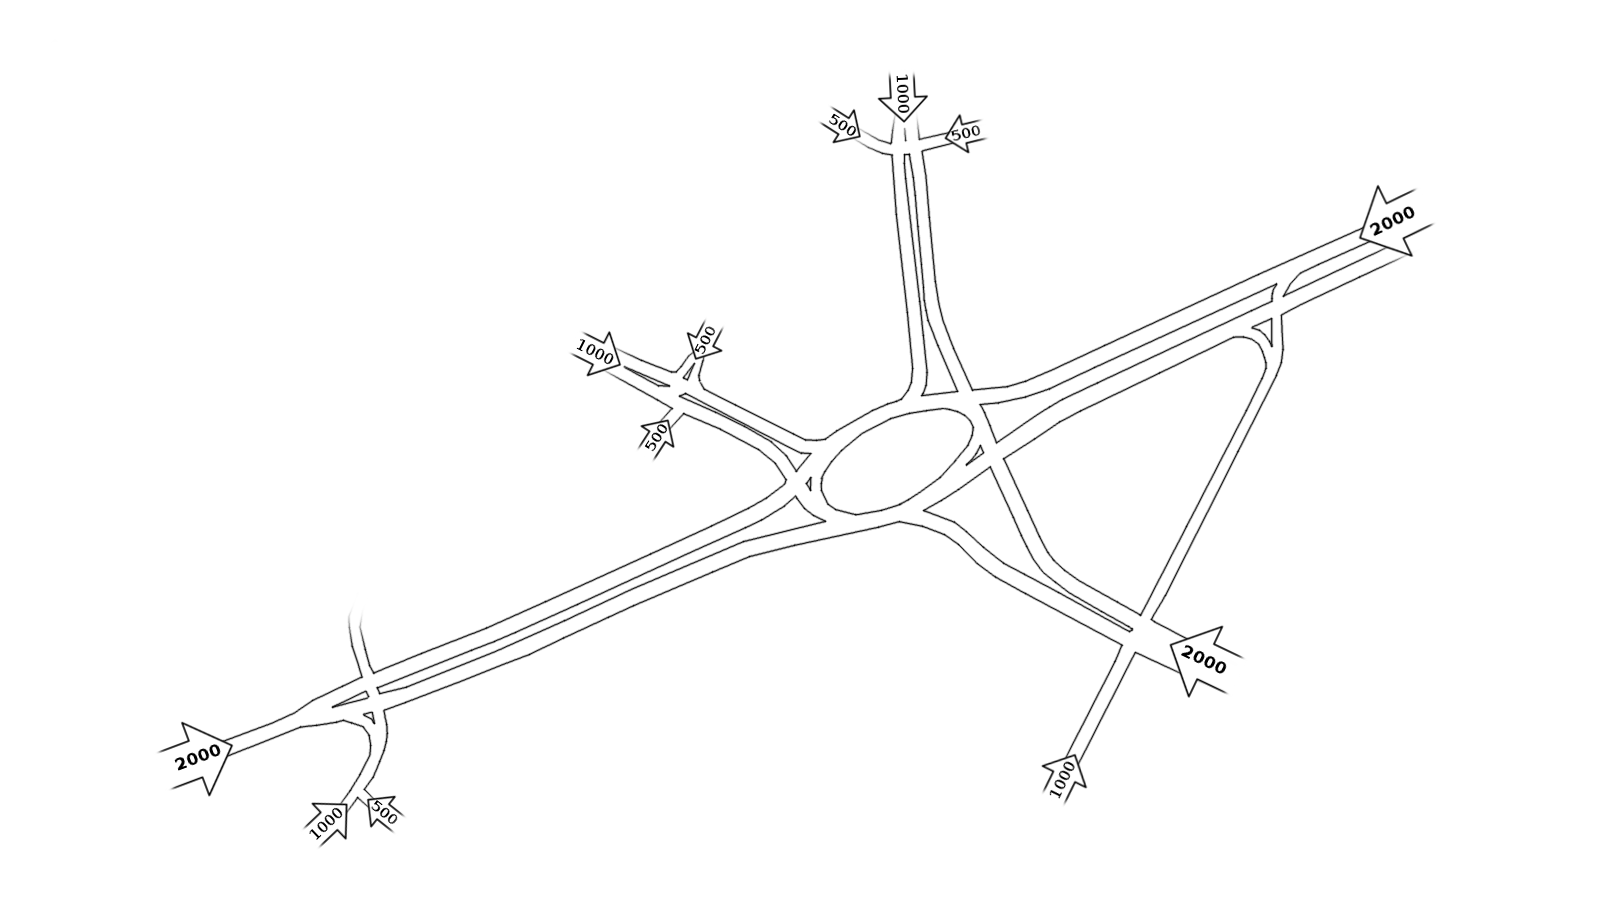
\includegraphics[width=1.0\textwidth]{images/mapa_ruch.png}
    \caption{Mapa przepływu pojazdów (w pojazdach na godzinę) w punktach wejściowych do sterowanego obszaru, przygotowana na podstawie Google Maps \cite{google_maps}}
    \label{fig:mapa_ruch}
\end{figure}

Na potrzeby symulacji ruchu na przedstawionym obszarze model NaSch został zmodyfikowany w celu przystosowania go do działania z przecinającym się ruchem na skrzyżowaniach i obsługę sterowania ruchem. Model został zmodyfikowany poprzez:
\begin{itemize}
	\item usunięcie fazy losowości ze względu na chęć badania reakcji ruchu na zmiany w sterowaniu nie losową charakterystykę ruchu,
	\item wprowadzenie elementów tworzących pojazdy zgodnie z przyjętym przepływem na punktach wejściowych do sterowanego obszaru,
	\item dodanie możliwości sterowania sygnałem zezwalającym na opuszczenie komórki i reakcja pojazdów na nadawane synały,
	\item modyfikacja fazy spowolnienia dla uwzględnienia konieczności zatrzymania się przed przecinającym strumieniem ruchu, w celu eliminacji blokowania innych pojazdów,
\end{itemize}

Ze względu na przedstawione ogranicznia symulatora, przyjęte zostały orientancyjne wartości przepływów pojazdów w punktach wejściowych, przedstawione na rysunku \ref{fig:mapa_ruch}.

Symulatowane są również czujniki ruchu. Czujnik przepływu pojazdów oblicza aktualny przepływ pojazdów na podstawie liczby pojazdów które przecięły określoną komórkę w ciągu ostatnich 10 sekund (jest to parametr konfiguracyjny symulatora). Czujnik kolejki określa wielkość kolejki na wyznaczonym odcinku, przez zliczenie liczby pojazdów znajdujących się w komórkach danego odcinka. Symulowane czujniki odzwierciedlają kamery z oprogramowaniem pozwalającym na wykrywanie pojazdów i pętle indukcyjne montowane w jezdni.

Symulator jest głównym źródłem czasu dla pozostałych komponentów systemu. Udostępnia on sygnał zegarowy o okresie jednej sekundy co wyzwala wyznaczenie nowego stanu sygnalizatorów przez kontrolery. Sygnał zegarowy jest odpowiednikiem sygnału 1PPS\footnote{one pulse per second (jeden impuls na sekundę) - elektroniczny sygnał synchronizacyjny, udostępniany między innymi przez satelity GPS} stosowanego powszechnie do synchronizacji działania układów elektronicznych.

\section{Kontroler}
\label{chap:kontroler}
Kontroler został przygotowany do działania z różnymi, prostymi w modyfikacji, algorytmami sterowania. Zmiana wybranego algorytmu spośród zaimplementowanych odbywa się poprzez edycję pliku konfiguracyjnego. Dla celu badań przygotowany został, poza opisanym algorytmem, algorytm sterowania przy użyciu stałoczasowego, wczytywanego z pliku, programu sygnalizacji.

\section{Komunikacja}
\label{chap:komunikacja}
Symulowany system sterowania ruchem wykorzystuje komunikację sieciową do połączenia komponentów. W założeniu wdrożony system wykorzystywałby czujniki i kontrolery komunikujące się przy użyciu sieci ethernet. Przygotowany, symulowany, system wykorzystuje do komunikacji centralny serwer odpowiedzialny za wymianę zdarzeń pomiędzy komponentami przy użyciu dyspozytora zdarzeń. Komunikacja sieciowa odbywa się przy użyciu biblioteki protobuf \cite{protobuf} w celu serializacji i deserializacji wiadomości.

\chapter{Ocena działania algorytmu}
\label{chap:ocena}
Na przygotowanym systemie przeprowadzone zostały badania z wykorzystaniem ruchu drogowego o przepływach przedstawionych na rysunku \ref{fig:mapa_ruch}. Każda konfiguracja była badana przez jedną godzinę, a wielkości badane to: średnia liczba zatrzymań pojazdów, średnia prędkość pojazdów oraz średnie czasy przejazdu na trzech, wybranych, trasach, przedstawionych na rysunku \ref{fig:mapa_trasy}.

\section{Wyniki badań}
W tabeli \ref{tab:predkosc} przedstawione zostały wartości średniej liczby zatrzymań i średniej prędkości w zależności od typu i parametrów sterowania.

\FloatBarrier
\begin{table}[h]
	\centering
	\begin{tabular}{ |r|c|c| }
		\hline
		& średnia liczba zatrzymań & średnia prędkość \\
		\hline
		brak kontroli                             & 33,01 & 12,02 km/h \\
		\hline
		stałoczasowa                              & 16,57 &  6,35 km/h \\
		\hline
		dynamiczna, 60s, p=0,33, q=0,33, r=0,33   & 11,00 &  9,32 km/h \\
		\hline
		dynamiczna, 90s, p=0,33, q=0,33, r=0,33   &  9,39 &  9,68 km/h \\
		\hline
		dynamiczna, 120s, p=0,33, q=0,33, r=0,33  &  8,30 &  9,70 km/h \\
		\hline
		dynamiczna, 120s, p=0,5, q=0,25, r=0,25   &  8,32 &  9,17 km/h \\
		\hline
		dynamiczna, 120s, p=0,8, q=0,1, r=0,1     &  8,38 &  9,15 km/h \\
		\hline
		dynamiczna, 120s, p=0,25, q=0,5, r=0,25   &  8,29 &  9,73 km/h \\
		\hline
		dynamiczna, 120s, p=0,1, q=0,8, r=0,1     & 11,54 &  8,85 km/h \\
		\hline
		dynamiczna, 120s, p=0,25, q=0,25, r=0,5   &  9,45 &  9,34 km/h \\
		\hline
		dynamiczna, 120s, p=0,1, q=0,1, r=0,8     & 10,72 &  9,35 km/h \\
		\hline
	\end{tabular}
	\caption{Zależność średniej liczby zatrzymań i średniej prędkości od typu i parametrów sterowania, p - wpływ przewidywanego przepływu pojazdów na sterowanie, q - wpływ aktualnego przepływu pojazdów na sterowanie, r - wpływ aktualnej wielkości kolejek na sterowanie}
	\label{tab:predkosc}
\end{table}
\FloatBarrier
\begin{figure}[h]
    \centering
    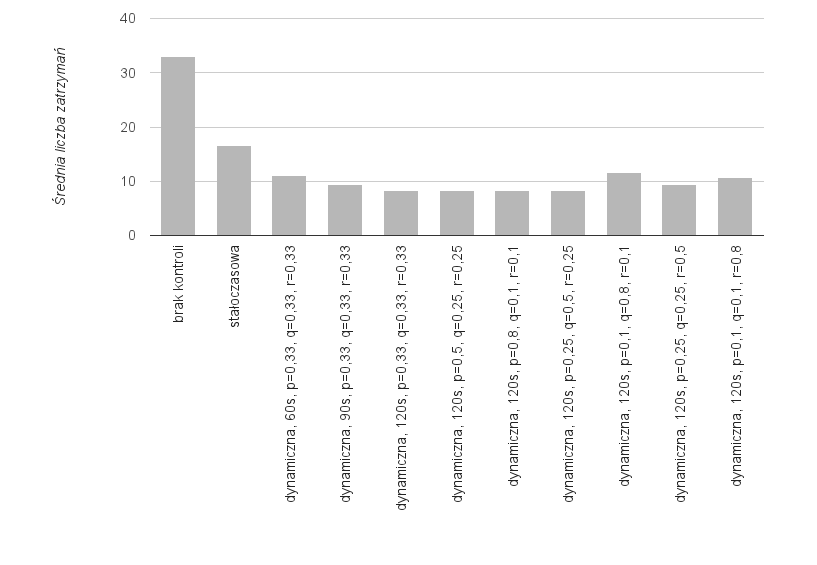
\includegraphics[width=1.0\textwidth]{images/wykres_liczba_zatrzyman.png}
    \caption{Wykres zależności średniej liczby zatrzymań od typu i parametrów sterowania}
    \label{fig:wykres_liczba_zatrzyman}
\end{figure}
\FloatBarrier

Na wykresie średniej liczby zatrzymań (rys. \ref{fig:wykres_liczba_zatrzyman}) możemy zaobserwować podstawową różnicę charakterystyki ruchu sterowanego i nie sterowanego.
Niekontrolowany ruch wykazuje się dużą, w porównaniu z pozostałymi badanymi konfiguracjami, liczbą zatrzymań co może być spowodowane skokowym ruchem pojazdów czekających na przejazd, na przykład wyjeżdżających z ulicy podporządkowanej. Jest to analogiczne z ruchem pojazdów poruszających się w korku i często przejeżdżającymi zaledwie kilka metrów.

Badany algorytm dynamiczny charakteryzuje się również lepszą, mniejszą, liczbą zatrzymań pojazdów niż stałoczasowy program sygnalizacji.
Spośród badanych wartości parametrów, najlepsza wydaje się konfiguracja podstawowa, o równej wielkości badanych parametrów, oraz konfiguracja faworyzująca spodziewany przepływ pojazdów otrzymany od sąsiadujących kontrolerów. Większa długość cyklu uzyskuje lepsze wyniki ze względu na rzadszą, wymuszoną, zmianę świateł.

\FloatBarrier
\begin{figure}[h]
    \centering
    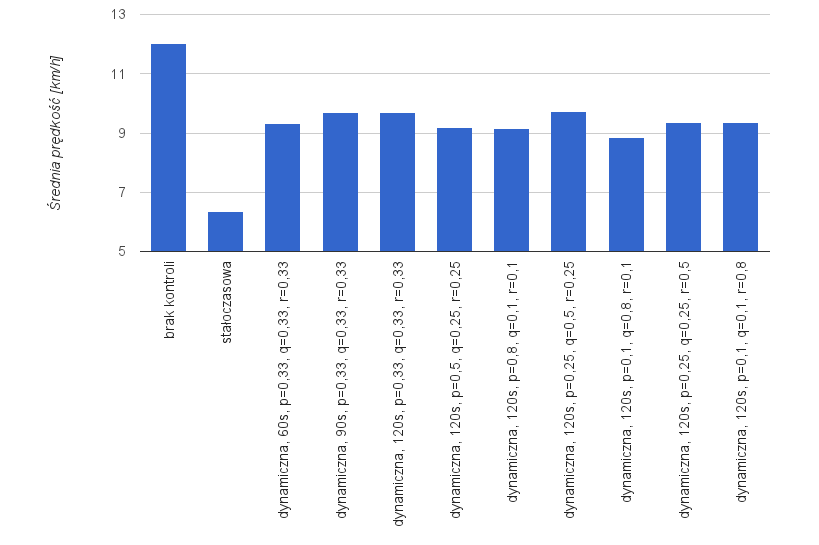
\includegraphics[width=1.0\textwidth]{images/wykres_predkosc.png}
    \caption{Wykres zależności średniej prędkości od typu i parametrów sterowania}
    \label{fig:wykres_predkosc}
\end{figure}
\FloatBarrier

Wykres średniej prędkości pojazdów (rys. \ref{fig:wykres_predkosc}) ukazuje wpływ układu drogowego, w szczególności drogi głównej, na prędkość średnią całego układu w przypadku braku sterowania. W badanym układzie drogowym droga główna znajduje się pomiędzy obszarami określonymi na rysunku \ref{fig:mapa_czysta} jako most Grunwaldzki i plac Grunwaldzki. Jest to droga o dużym natężeniu ruchu co powoduje duży przepływ pojazdów na wspomnianej relacji i zwiększa średnią prędkość pojazdów.

Najgorszą, najmniejszą, wielkością charakteryzuje się stałoczasowy program sygnalizacji, który najbardziej ogranicza średnią prędkość pojazdów.

Badany algorytm sterowania uzyskuje pośrednie wyniki, ze wskazaniem na równe wartości parametrów. Studwudziesto sekundowy cykl również w tym przypadku uzyskuje lepsze wyniki niż krótszy cykl.

\FloatBarrier
\begin{figure}[h]
    \centering
    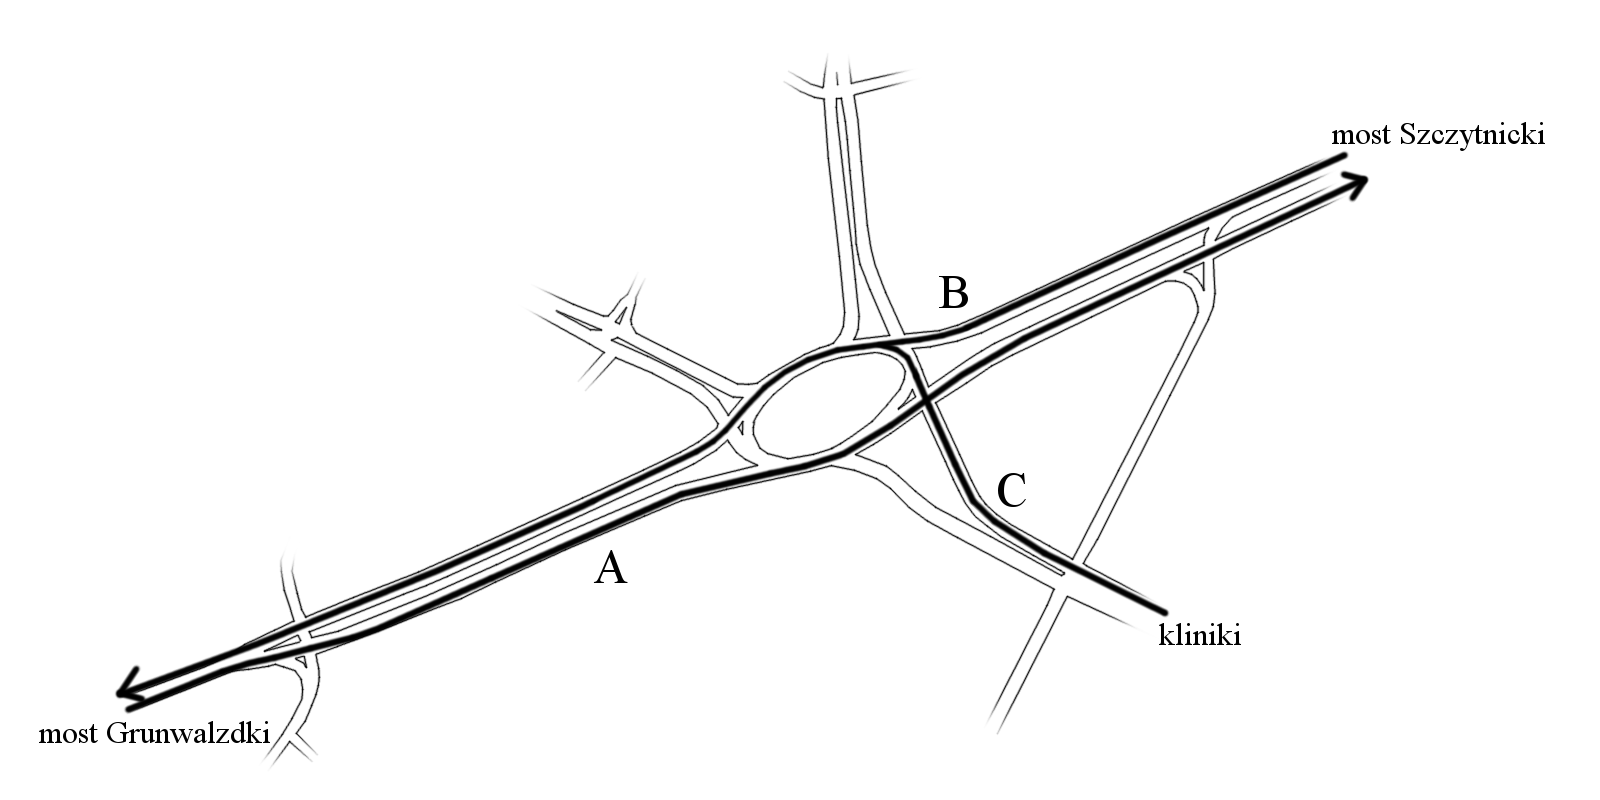
\includegraphics[width=1.0\textwidth]{images/mapa_trasy.png}
    \caption{Mapa przedstawiająca badane trasy przejazdu, przygotowana na podstawie Google Maps \cite{google_maps}}
    \label{fig:mapa_trasy}
\end{figure}
\FloatBarrier

W dalszej części badane były czasy przejazdu na trzech wybranych trasach, przedstawionych na rysunku \ref{fig:mapa_trasy}.
Trasa A, z mostu Grunwaldzkiego w kierunku mostu Szczytnickiego, oraz trasa B, z kierunku mostu Szczytnickiego do mostu Grunwaldzkiego jest wspomnianą wcześniej drogą główną, na której opóźnienia, w przypadku braku sterowania, powstają ze względu na tworzenie się korków przy zjeździe z niej. Trasa C z klinik (ulica Skłodowskiej-Curie) do mostu Grunwaldzkiego jest trasą podporządkowaną przez co ruch na niej zależy w dużym stopniu od ruchu na dwóch pozostałych trasach.

\FloatBarrier
\begin{figure}[h]
    \centering
    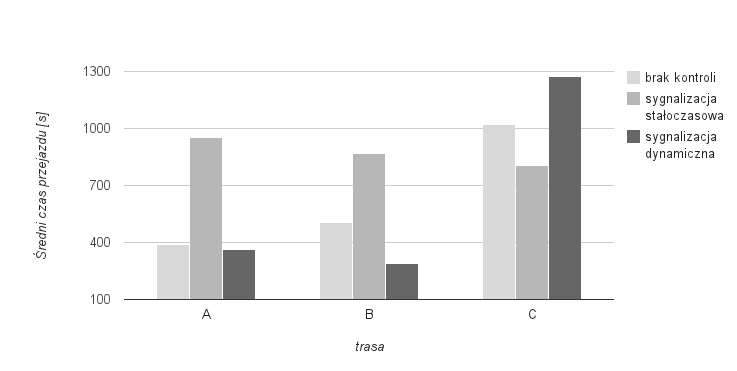
\includegraphics[width=1.0\textwidth]{images/wykres_typ_sterowania_czas.png}
    \caption{Wykres zależności średniego czasu przejazdu od typu sterowania}
    \label{fig:wykres_typ_sterowania_czas}
\end{figure}
\FloatBarrier
\begin{table}[h]
	\centering
	\begin{tabular}{ |r|c|c|c| }
		\hline
		& trasa A & trasa B & trasa C \\
		\hline
		brak kontroli & 389,58 s & 504,49 s & 1019,22 s \\
		\hline
		sygnalizacja stałoczasowa & 951,87 s & 867,70 s & 806,33 s \\
		\hline
		sygnalizacja dynamiczna & 365,05 s & 288,85 s & 1273,50 s \\
		\hline
	\end{tabular}
	\caption{Zależność średniego czasu przejazdu od typu sterowania}
	\label{tab:wykres_typ_sterowania_czas}
\end{table}
\FloatBarrier
Przedstawione na wykresie \ref{fig:wykres_typ_sterowania_czas} i w tabeli \ref{tab:wykres_typ_sterowania_czas} średnie czasy przejazdu na wybranych trasach przedstawiają podstawowe róznice w sterowaniu stałoczasowym o stałym programi i sterowaniu dynamicznym. Sterowanie stałoczasowe charakteryzuje się wyrównaniem czasów przejazdu na wybranych trasach, co w przypadku trasy C daje zdecydowaną poprawę.

Badany algorytm dynamiczny wykazuje poprawę w przypadku tras A i B, jednak powoduje również pogorszenie sytuacji dla trasy C. Może to być spowodowane metodą wyznaczania następnego stanu sterowania. Wyliczana jest suma wag poszczególnych sygnalizatorów. Natomiast w dojeździe do punktu kolizji trasy C z trasami A i B, trasa C posiada 3 sygnalizatory natomiast A i B posiadają 6 sygnalizatorów na niekolidujących strumieniach ruchu.

\FloatBarrier
\begin{figure}[h]
    \centering
    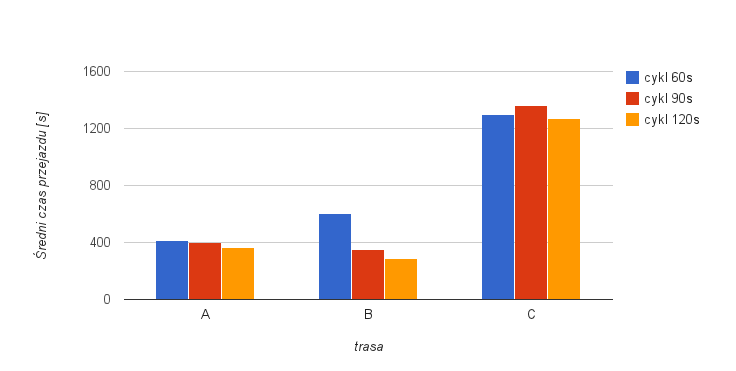
\includegraphics[width=1.0\textwidth]{images/wykres_dlugosc_cyklu_czas.png}
    \caption{Wykres zależności średniego czasu przejazdu od długości cyklu w sygnalizacji dynamicznej}
    \label{fig:wykres_dlugosc_cyklu_czas}
\end{figure}
\FloatBarrier
\begin{table}[h]
	\centering
	\begin{tabular}{ |r|c|c|c| }
		\hline
		& trasa A & trasa B & trasa C \\
		\hline
		cykl 60 s & 412,72 s & 602,86 s & 1301,70 s \\
		\hline
		cykl 90 s & 398,09 s & 353,62 s & 1361,07 s \\
		\hline
		cykl 120 s & 365,05 s & 288,85 s & 1273,50 s \\
		\hline
	\end{tabular}
	\caption{Zależność średniego czasu przejazdu od długości cyklu w sygnalizacji dynamicznej}
	\label{tab:wykres_dlugosc_cyklu_czas}
\end{table}
\FloatBarrier
Na wykresie \ref{fig:wykres_dlugosc_cyklu_czas} i w tabeli \ref{tab:wykres_dlugosc_cyklu_czas} widzimy zależność czasu przejazdu od długości cyklu. W tym przypadku, podobnie jak dla wartości średniej liczby zatrzymań i prędkości przedstawionych w tabeli \ref{tab:predkosc}, lepsze wyniki uzyskuje większa długość cyklu świetlnego.

\FloatBarrier
\begin{figure}[h]
    \centering
    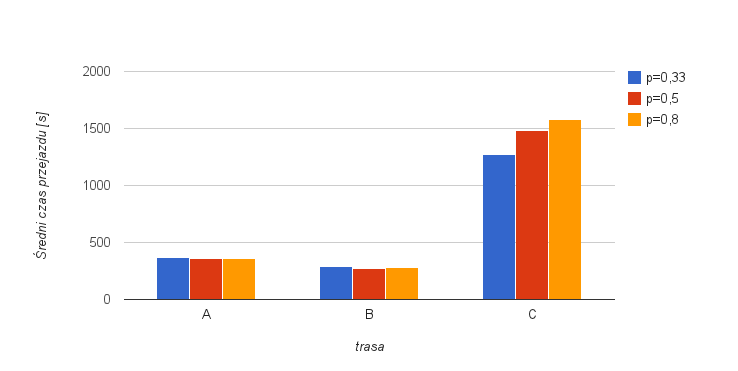
\includegraphics[width=1.0\textwidth]{images/wykres_przewidywany_przeplyw_czas.png}
    \caption{Wykres zależności średniego czasu przejazdu od wpływu (p) przewidywanego przepływu na sterowanie w sygnalizacji dynamicznej}
    \label{fig:wykres_przewidywany_przeplyw_czas}
\end{figure}
\FloatBarrier
\begin{table}[h]
	\centering
	\begin{tabular}{ |r|c|c|c| }
		\hline
		& trasa A & trasa B & trasa C \\
		\hline
		p=0,33 & 365,05 s & 288,85 s & 1273,50 s \\
		\hline
		p=0,5 & 356,70 s & 272,23 s & 1484,91 s \\
		\hline
		p=0,8 & 361,30 s & 279,42 s & 1581,82 s \\
		\hline
	\end{tabular}
	\caption{Zależność średniego czasu przejazdu od wpływu (p) przewidywanego przepływu na sterowanie w sygnalizacji dynamicznej}
	\label{tab:wykres_przewidywany_przeplyw_czas}
\end{table}
\FloatBarrier
Wykres \ref{fig:wykres_przewidywany_przeplyw_czas} i tabela \ref{tab:wykres_przewidywany_przeplyw_czas} przedstawia zależność wpływu przewidywanego przepływu na sterowanie. Widzimy że zwiększenie wielkości badanego parametru do wielkości q=0,5 powoduje poprawę czasu przejazdu dla tras A i B. Dalsze zwiększanie wielkości parametru zmienjsza efektywność. W przypadku trasy C można zaobserwować zwiększenie czasu przjazdu przy zwiększaniu wartości parametru.

\FloatBarrier
\begin{figure}[h]
    \centering
    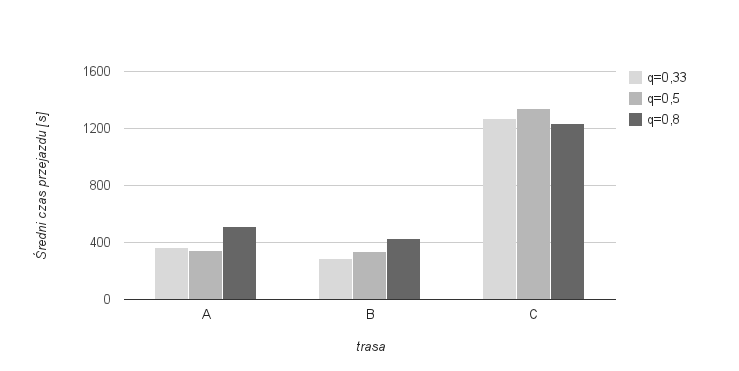
\includegraphics[width=1.0\textwidth]{images/wykres_przeplyw_czas.png}
    \caption{Wykres zależności średniego czasu przejazdu od wpływu (q) aktualnego przepływu na sterowanie w sygnalizacji dynamicznej}
    \label{fig:wykres_przeplyw_czas}
\end{figure}
\FloatBarrier
\begin{table}[h]
	\centering
	\begin{tabular}{ |r|c|c|c| }
		\hline
		& trasa A & trasa B & trasa C \\
		\hline
		q=0,33 & 365,05 s & 288,85 s & 1273,50 s \\
		\hline
		q=0,5 & 344,73 s & 337,45 s & 1341,16 s \\
		\hline
		q=0,8 & 511,69 s & 429,03 s & 1236,22 s \\
		\hline
	\end{tabular}
	\caption{Zależność średniego czasu przejazdu od wpływu (q) aktualnego przepływu na sterowanie w sygnalizacji dynamicznej}
	\label{tab:wykres_przeplyw_czas}
\end{table}
\FloatBarrier
Kolejny wykres (\ref{fig:wykres_przeplyw_czas}) przedstawia zależność czasu przejazdu od aktualnego przepływu pojazdów. W przypadku zwiększenia tego parametru, do wartości 0,5, możemy zaobserwować minimalną poprawę dla trasy A, przy dalszym zwiększaniu wartości parametru wynik pogarsza się.
Widać również pewną poprawę wyniku dla trasy C i wartości parametru 0,8.
Znaczenie tego parametru może być pomniejszone, przy wykonanych badaniach z wykorzystaniem dużego ruchu, ze względu na zmniejszenie przepływu w przypadku powstania korku. Zarówno pojazdy stojące w korku jak i brak pojazdów będzie odznaczał się wielkością przepływu 0 pojazdów na godzinę.

\FloatBarrier
\begin{figure}[h]
    \centering
    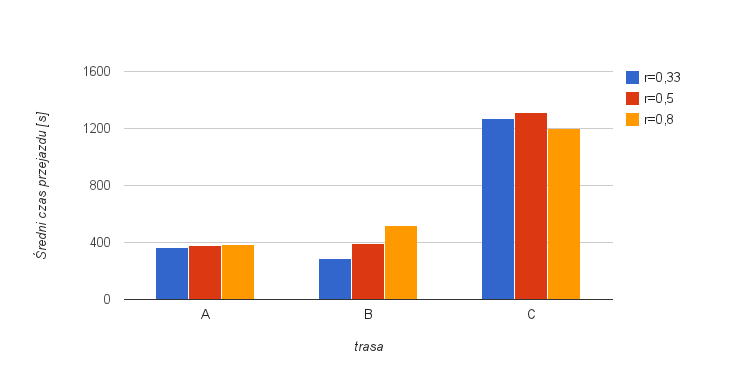
\includegraphics[width=1.0\textwidth]{images/wykres_kolejka_czas.png}
    \caption{Wykres zależności średniego czasu przejazdu od wpływu (r) aktualnej kolejki na sterowanie w sygnalizacji dynamicznej}
    \label{fig:wykres_kolejka_czas}
\end{figure}
\FloatBarrier
\begin{table}[h]
	\centering
	\begin{tabular}{ |r|c|c|c| }
		\hline
		& trasa A & trasa B & trasa C \\
		\hline
		r=0,33 & 365,05 s & 288,85 s & 1273,50 s \\
		\hline
		r=0,5 & 378,00 s & 392,09 s & 1314,89 s \\
		\hline
		r=0,8 & 385,92 s & 517,71 s & 1200,47 s \\
		\hline
	\end{tabular}
	\caption{Zależność średniego czasu przejazdu od wpływu (r) aktualnej kolejki na sterowanie w sygnalizacji dynamicznej}
	\label{tab:wykres_kolejka_czas}
\end{table}
\FloatBarrier
Na wykresie \ref{fig:wykres_kolejka_czas} i w tabeli \ref{tab:wykres_kolejka_czas} przedstawiona została zależność czasu przejazdu od wpływu aktualnej kolejki na sterowanie. Można zaobserwować, że zwiększenie wpływu kolejki na sterowanie powoduje zwiększenia czasu przejazdu na drodze głównej (trasach A i B). Jednocześnie dla wielkości parametru 0,8 czas przejazdu na trasie podporządkowanej zmniejszył się.
Podobnie jak w przypadku przepływu pojazdów, działanie tego parametru jest ograniczone w obciążonej sieci drogowej. Ze względu na normalizację kolejek, gdy są one pełne, ich wielkości będą, z punktu widzenia algorytmu, równe.

\chapter{Wnioski}
TODO wnioski, propozycje rozwoju

%\chapter{Dummy Rozdział}
Lorem ipsum dolor sit amet, consectetur adipiscing elit. Etiam fermentum hendrerit risus nec ultrices. Sed adipiscing adipiscing nunc, non convallis mauris facilisis nec. Nunc lorem elit, viverra vitae neque et, commodo egestas enim. Proin a ante non leo consequat lobortis hendrerit ut nisl. Phasellus quis feugiat urna, sit amet rutrum sem. Pellentesque habitant morbi tristique senectus et netus et malesuada fames ac turpis egestas. Donec a mattis nulla, et tincidunt purus. Etiam et sagittis tortor, ut venenatis eros. Nullam vulputate scelerisque molestie. Sed consequat ipsum et gravida viverra. Phasellus nec congue augue. Aenean pretium erat elit, eget pretium erat vulputate ut. Pellentesque porta imperdiet ante, vel pellentesque est lobortis convallis. Curabitur at augue tincidunt velit dictum pellentesque sit amet in massa. Dane znajdują się w tabeli ~\ref{tab:testowa} na stronie ~\pageref{tab:testowa}.
\begin{table}[h] %h - here - nie do końca ale działa
	\caption{A normal caption}
	\begin{tabular}{ r|c|c| }
		\multicolumn{1}{r}{}
 		&  \multicolumn{1}{c}{noninteractive}
 		& \multicolumn{1}{c}{interactive} \\
		\cline{2-3}
		massively multiple & Library & University \\
		\cline{2-3}
		one-to-one & Book & Tutor \\
		\cline{2-3}
	\end{tabular}
	\caption*{na podstawie http://costam.pl}
	\label{tab:testowa}
\end{table}
test %\cite{abramowitz+stegun}
Lorem ipsum dolor sit amet, consectetur adipiscing elit. Etiam fermentum hendrerit risus nec ultrices. Sed adipiscing adipiscing nunc, non convallis mauris facilisis nec. Nunc lorem elit, viverra vitae neque et, commodo egestas enim. Proin a ante non leo consequat lobortis hendrerit ut nisl. Phasellus quis feugiat urna, sit amet rutrum sem. Pellentesque habitant morbi tristique senectus et netus et malesuada fames ac turpis egestas. Donec a mattis nulla, et tincidunt purus. Etiam et sagittis tortor, ut venenatis eros. Nullam vulputate scelerisque molestie. Sed consequat ipsum et gravida viverra. Phasellus nec congue augue. Aenean pretium erat elit, eget pretium erat vulputate ut. Pellentesque porta imperdiet ante, vel pellentesque est lobortis convallis. Curabitur at augue tincidunt velit dictum pellentesque sit amet in massa.

Lorem ipsum dolor sit amet, consectetur adipiscing elit. Etiam fermentum hendrerit risus nec ultrices. Sed adipiscing adipiscing nunc, non convallis mauris facilisis nec. Nunc lorem elit, viverra vitae neque et, commodo egestas enim. Proin a ante non leo consequat lobortis hendrerit ut nisl. Phasellus quis feugiat urna, sit amet rutrum sem. Pellentesque habitant morbi tristique senectus et netus et malesuada fames ac turpis egestas. Donec a mattis nulla, et tincidunt purus. Etiam et sagittis tortor, ut venenatis eros. Nullam vulputate scelerisque molestie. Sed consequat ipsum et gravida viverra. Phasellus nec congue augue. Aenean pretium erat elit, eget pretium erat vulputate ut. Pellentesque porta imperdiet ante, vel pellentesque est lobortis convallis. Curabitur at augue tincidunt velit dictum pellentesque sit amet in massa.

Lorem ipsum dolor sit amet, consectetur adipiscing elit. Etiam fermentum hendrerit risus nec ultrices. Sed adipiscing adipiscing nunc, non convallis mauris facilisis nec. Nunc lorem elit, viverra vitae neque et, commodo egestas enim. Proin a ante non leo consequat lobortis hendrerit ut nisl. Phasellus quis feugiat urna, sit amet rutrum sem. Pellentesque habitant morbi tristique senectus et netus et malesuada fames ac turpis egestas. Donec a mattis nulla, et tincidunt purus. Etiam et sagittis tortor, ut venenatis eros. Nullam vulputate scelerisque molestie. Sed consequat ipsum et gravida viverra. Phasellus nec congue augue. Aenean pretium erat elit, eget pretium erat vulputate ut. Pellentesque porta imperdiet ante, vel pellentesque est lobortis convallis. Curabitur at augue tincidunt velit dictum pellentesque sit amet in massa.

\pagestyle{plain}
%\pagenumbering{gobble}

%\listoffigures
%\listoftables

\bibliographystyle{iisthesis}
\bibliography{biblio}

\appendix
%\chapter{Wykorzystane pojęcia}

\begin{description}

\item[autonomiczna część skrzyżowania] --
część skrzyżowania, w której dojazd potoków ruchu do miejsca przecięcia jest kontrolowany
jedynie przez sygnalizatory znajdujące się w danej części skrzyżowania

\item[chwila czasu] -- TODO

\item[czujnik] -- TODO

\item[kontroler] -- TODO

\item[obszar sterowania] --
obszar, obejmujący pojedyncze skrzyżowanie lub autonomiczną część skrzyżowania,
kontrolowany przez pojedynczy kontroler

\end{description}

\chapter{Materiały załączone w formie elektronicznej}

Załączona płyta zawiera kopię repozytorium pracy magisterskiej.

\begin{description}

\item[katalog 3rdparty] --
biblioteki potrzebne do skompilowania przygotowanego systemu

\item[katalog tex] --
tekst pracy magisterskiej w formacie \LaTeX

\item[katalog thesis] --
kod źródłowy przygotowanego systemu

\item[plik praca\_dyplomowa.pdf] --
tekst pracy magisterskiej w formacie pdf


\end{description}

\end{document}

